\documentclass[runningheads]{llncs}

% ---------- PACKAGES ----------
\usepackage[utf8]{inputenc}
\usepackage{graphicx}
\usepackage{amsmath, amssymb}
\usepackage{booktabs}
\usepackage{multirow}
\usepackage{tabularx}
\usepackage{float}
\usepackage{caption}
\usepackage{subcaption}
\usepackage{lipsum}
\usepackage{url}
\usepackage{cite}
\usepackage{url}
\usepackage{enumitem} % đặt ở phần đầu file
\usepackage{placeins}
\usepackage{booktabs}   % kẻ bảng đẹp


% ---------- TABLE ADJUSTMENT ----------
\usepackage{adjustbox}
\usepackage{longtable}  % Nếu cần bảng nhiều dòng
\usepackage{stfloats}   % Cho phép table* nằm dưới cuối trang
% ---------- BEGIN DOCUMENT ----------
\begin{document}

% ---------- TITLE ----------
\title{Developing a Machine Learning-Based Tool for Autism Screening Using Psychological Medical Records}

\author{Hao Nguyen Thi Bich\inst{1} \and
Thanh Nguyen Van Quoc\inst{2} \and
Nhut Nguyen Minh\inst{3} \and
Thuan Nguyen Dinh\inst{4}}
\authorrunning{Nguyen T.B. Hao, Nguyen V.Q. Thanh, Nguyen M. Nhut, Nguyen D. Thuan}


\institute{Faculty of Information Systems, University of Information Technology - Vietnam National University, Ho Chi Minh City, Vietnam\\
\email{\{21521447@gm.uit.edu.vn, 21522049@gm.uit.edu.vn, nhutnm.17@grad.uit.edu.vn, thuannd@uit.edu.vn\}}}

\maketitle

% ---------- ABSTRACT ----------
\begin{abstract}
Autism Spectrum Disorder (ASD) is a neurodevelopmental condition that impacts social interaction and behavior, where early detection is crucial for optimizing intervention outcomes. This study proposes a machine learning-based screening tool that utilizes psychological medical records (EMR) to identify ASD in children aged 1 to 8 years. We conducted an experiment using two datasets: (1) a publicly available dataset from a prior study, consisting of approximately 300 records with information on ASD status and responses to 10 evaluation questions; and (2) an EMR dataset from a pediatric psychology clinic, comprising about 600 records that include assessments from parents through interviews and from clinicians via direct examinations. Both datasets were labeled by psychology experts based on evaluation criteria such as eye contact, pointing, imitation, and others.

The EMR dataset from the clinic includes 18 labeled features corresponding to evaluation criteria. For the public dataset, we analyzed the experimental questions and mapped them to the 18 features of the EMR dataset, selecting 10 statistically significant features. Both datasets underwent preprocessing to handle missing data, encode features, and select features with significant impact on the outcome label. This resulted in 10 key features used for training machine learning classification models.

Four machine learning models were implemented: Decision Tree, XGBoost, CatBoost, and Overall Local Accuracy (OLA). Results showed that OLA exhibited superior adaptability across both standard and potentially noisy datasets. However, initial experiments revealed two main challenges: (1) class imbalance (90\% ASD vs. 10\% non-ASD), and (2) feature bias due to the high accuracy of expert-labeled EMR data, causing models to over-rely on certain features. These limitations reduced the models’ reliability in real-world applications.

To address these issues, we applied the SMOTE-IPF technique to balance the ASD and non-ASD class ratios and enhanced the OLA framework by incorporating dynamic weighting and regularization to reduce dependency on specific features. The improved models achieved an F1-Score of 0.89 and an AUC-ROC of 0.90, with significantly reduced feature bias, as evidenced by a more balanced distribution of feature importance. The proposed screening tool offers a cost-effective and scalable solution, particularly suitable for resource-constrained settings. It has the potential for further improvement through training on larger datasets, enhancing its ability to handle outliers and increasing overall accuracy.\end{abstract}

% ---------- KEYWORDS ----------
\keywords{Autism Spectrum Disorder, Machine Learning, Psychological Medical Records, SMOTE-IPF, OLA, Screening Tool}
\section{Introduction}
Autism Spectrum Disorder (ASD) is a neurodevelopmental condition characterized by challenges in social interaction, communication, and repetitive behaviors, affecting individuals across childhood, adolescence, and adulthood ~\cite{b1}. Early detection in children is critical for timely interventions that optimize long-term outcomes. However, as children age, diagnosis and intervention become increasingly complex due to overlapping symptoms with other mental health disorders. According to the U.S. Centers for Disease Control and Prevention (CDC), the prevalence of ASD in the United States has risen sharply from 1 in 150 children in 2000 to 1 in 36 in 2023~\cite{b2}. Similar trends are observed globally, some reported rates: 
\begin{itemize}
    \item Accounting for 1 in 57 in the United Kingdom
    \item Accounting for 1 in 100 in Japan 
    \item Accounting for 1 in 120 in China
\end{itemize}
In Vietnam, while official statistics are lacking, preliminary estimates suggest a prevalence of approximately 1 in 68 children, driven by increased societal awareness, improved diagnostic capabilities, and potential environmental and lifestyle factors.

Traditional screening tools, such as M-CHAT-R/F and ADOS, are resource-intensive, requiring specialized expertise and limiting their accessibility in low-resource settings, particularly in developing countries like Vietnam ~\cite{b3}. The absence of specific medical tests for ASD further complicates diagnosis, relying heavily on subjective observational assessments. Recent advancements in artificial intelligence (AI) and machine learning (ML) offer promising opportunities for automated ASD screening by leveraging electronic medical records (EMR). However, using EMR for ASD prediction remains a nascent field, particularly in contexts like Vietnam, where medical data is often heterogeneous, imbalanced (fewer ASD cases), and prone to feature bias (over-reliance on specific indicators) ~\cite{b4}. Previous ML studies have applied models like Decision Trees, XGBoost, and CatBoost, achieving high accuracy in controlled settings but struggling with real-world generalizability due to data imbalances and dominant features.

This study proposes an ML-based ASD screening tool utilizing psychological EMRs from children aged 1-8 years, addressing practical challenges such as class imbalance and feature bias. We evaluate four ML models-Decision Tree, XGBoost, CatBoost, and an enhanced Overall Local Accuracy (OLA) framework-introducing SMOTE-IPF for data augmentation and tailored adjustments to OLA to mitigate bias. Our contributions include: (1) a robust dataset combining 300 public records and 600 clinical EMRs, preprocessed with expert guidance; (2) an improved OLA framework for adaptive and unbiased predictions; and (3) a cost-effective, scalable tool tailored for resource-constrained settings. 

The paper is organized as follows: Section 2 reviews related work, Section 3 describes the datasets and preprocessing, Section 4 details the methodology, Section 5 presents experimental results and analysis, and Section 6 discusses contributions, limitations, and future directions.

\section{Related Works}

Harshita Chandrappa, Swaathi BR, Prof. Swimpy Pahuja.~\cite{b5} proposed a hybrid machine learning framework for predicting Autism Spectrum Disorder (ASD) across all age groups. The system incorporates multiple ML classifiers such as Decision Tree, Naive Bayes, Random Forest, SVM, and Logistic Regression into a web-based diagnostic application. Through preprocessing and classification on a structured ASD dataset, their approach demonstrated high accuracy in predicting ASD traits. Among the models evaluated, Support Vector Machine and Random Forest yielded the best results in terms of accuracy and robustness. The authors highlighted the importance of early screening and presented a chatbot-based interface to assist users in understanding ASD symptoms and diagnosis.

Jose A. Saez, Julian Luengo, Jerzy Stefanowski, Francisco Herrera ~\cite{b6} introduced SMOTE-IDF, a novel text classification method combining SMOTE oversampling with IDF weighting to tackle class imbalance in textual datasets. Using a Deep Neural Network (DNN) classifier, SMOTE-IDF balances minority class samples while preserving the significance of rare, informative terms. Tested on datasets like 20 Newsgroups, it outperformed traditional oversampling and baseline classifiers in accuracy, precision, recall, and F1-score, highlighting the value of hybrid sampling and feature weighting for imbalanced textual data.

Hanen Karamti, Raed Alharthi, Amira Al Anizi, Reemah M. Alhebshi, Ala’ Abdulmajid Eshmawi, Shtwai Alsubai, Muhammad Umer.~\cite{b7} introduced an enhanced oversampling technique named SMOTE-KNN, which improves upon the original SMOTE algorithm by integrating a K-Nearest Neighbors (KNN)-based adaptive mechanism. The proposed method dynamically selects appropriate neighbor samples for synthetic instance generation, aiming to reduce noise and overlap between classes in imbalanced datasets. The authors validated SMOTE-KNN on multiple benchmark datasets and compared its performance with traditional SMOTE, Borderline-SMOTE, and ADASYN. Experimental results demonstrated that SMOTE-KNN significantly enhances classification metrics such as precision, recall, and F1-score across various classifiers. The study underlines the importance of local data structure in oversampling and offers a more robust strategy for handling imbalance in binary classification problems.

B. D. Hung, V. V. Thoa, and X. T. Dang.~\cite{b8} introduced KSI, a novel hybrid method that combines clustering with SMOTE and iterative noise filtering (IPF) to enhance classification performance on imbalanced datasets. While traditional SMOTE and SMOTE-IPF approaches are commonly used for over-sampling minority classes, they often generate noisy or overlapping samples, reducing classification accuracy. KSI addresses this by using k-means clustering to identify local distributions where minority instances may dominate or be sparse. Synthetic samples are only generated in regions where local minority density is low, followed by IPF to remove noise. Experiments on multiple UCI datasets demonstrated that KSI outperforms baseline methods (SMOTE, IPF, SMOTE-IPF) in terms of G-mean and AUC, particularly on noisy and borderline samples.

Youngkyu Hong, Eunho Yang.~\cite{b9} proposed a dual-branch learning framework to address bias in image classification. It uses Bias-Contrastive Learning (BCL) to capture spurious correlations in a biased branch and Bias-Balanced Learning (BBL) to focus on robust features in an unbiased branch. By minimizing biased branch loss and maximizing unbiased branch agreement with true labels, the method reduces reliance on dataset biases, outperforming traditional debiasing techniques on datasets like Biased-MNIST and ImageNet-9.

Y. Zeng, J. Liu, H. Lam, and H. Namkoong.~\cite{b10} introduces Ola, an advanced omni-modal language model capable of understanding images, audio, and video. It uses progressive modality alignment-gradually learning from image-text, audio, then video-to reduce training costs. Ola supports streaming speech generation and demonstrates state-of-the-art performance among open-source omni-modal models, rivaling specialized systems across diverse tasks.

\section{Dataset}
This section provides an overview of the datasets employed in the research, offering insights into their composition, size, and the practical processes involved in their collection from real-world sources. To comprehensively evaluate the proposed approach, two datasets were utilized.
\subsection{Public Dataset}
The public dataset was sourced from Kaggle \cite{b17}, consisting of responses to 10 behavioral screening questions designed to detect ASD symptoms in children. The dataset is balanced, with an approximately equal distribution between ASD and non-ASD labels, each record includes binary responses to 10 questions, personal information and other relevant details. These 10 questions in the dataset are labeled to correspond with evaluation topic, which also support the labeling of the private dataset under the guidance and verification of psychological experts.
\begin{itemize}
    \item Total samples: 292 records
    \item Class distribution: 141/292 records ASD about 48,3\% 
    \item Number and types of features: 20 columns included raw columns and label columns
\end{itemize}

\subsection{Private Dataset}The private dataset was collected from the medical records of the Psychology Clinic, featuring a more complex structure and class imbalance due to medical records in favor of disease data. It contains over 600 samples, with richer information such as personal information, acknowledging behavior from relatives of children and evaluating from a specialist after a direct examination at the clinic. A major challenge in this dataset is the excessive dominance of a single feature, which represents the standard assessment by doctors. This feature exhibits a bias tendency, affecting the final clinical outcomes and resulting in model decisions with high experimental accuracy but prone to misapplication in practical settings.
\subsubsection{\textbf{Step 1:} Collect raw data} This study utilizes a dataset comprising over 1,200 pediatric psychological records collected from a child psychology clinic, covering various conditions such as Autism Spectrum Disorder (ASD), intellectual developmental disorder, language disorder, and attention deficit hyperactivity disorder. The initial step involved standardizing the data by converting PDF records into structured Excel tables. The records were then categorized by condition, resulting in the selection of over 800 cases related to ASD and non-clinical cases.
\subsubsection{\textbf{Step 2:} Filter data} Records with missing or substandard data were filtered out, yielding a refined dataset of about 600 records. Then, data labeling was performed to assign features known to influence ASD prediction, including eye contact~\cite{b11}, pointing gestures~\cite{b12}, response to name~\cite{b13}, joint attention~\cite{b14}, imitation~\cite{b15}, and symbolic play~\cite{b16}... These behavioral indicators were selected based on their strong association with early autism markers and clinical diagnostic standards. To ensure privacy, personal information was anonymized through encoding before further preprocessing.
\subsubsection{\textbf{Step 3:} Prepare dataset}
\begin{itemize}
    \item Number of samples: 594 records
    \item Class distribution: 550/594 records ASD-Tracking and ASD about 93\%
    \item Number and types of features: 36 columns included raw columns and label columns
\end{itemize}
\subsection{Summary Dataset}

The research utilized two datasets to evaluate an ASD detection approach. The public dataset from Kaggle contains 292 balanced records with 20 features, including 10 binary behavioral responses. The private dataset, collected from a psychology clinic, comprises 594 records with 36 features, predominantly ASD cases (93\%), derived from standardized medical records.

These datasets have 18 labeled features that are used for analysis and predict. These labeled features are listed below:
\newcounter{attr}       % bộ đếm cho cột ID
\newcommand{\attrrow}[1]{%
  \stepcounter{attr}\theattr & #1 \\ }  % macro sinh 1 dòng

\begin{table}[htbp]
  \centering
  \caption{List of labeled features in the dataset}
  \begin{tabular}{@{}ll@{}}
    \toprule
    \textbf{ID} & \textbf{Labeled Features Description} \\ \midrule
    \attrrow{Medical History}
    \attrrow{Speech Delay}
    \attrrow{Behavioral Rigidity}
    \attrrow{Behavioral Isolation }
    \attrrow{Sensorimotor Play}
    \attrrow{Functional Play}
    \attrrow{Combinatorial Play}
    \attrrow{Symbolic Play}
    \attrrow{Repetitive/Stereotyped Play}
    \attrrow{Social Communication Skills}
    \attrrow{Turn-Taking Play}
    \attrrow{Imitation}
    \attrrow{Task Requesting}
    \attrrow{Response to Name in Infants}
    \attrrow{Toe Walking after 3 years}
    \attrrow{Making a Point}
    \attrrow{Joint Attention}
    \attrrow{Eye Contact } \\ \bottomrule
  \end{tabular}
\end{table}

\section{Proposed Methodology}
This section outlines the proposed methodology for developing an Autism Spectrum Disorder (ASD) screening tool, detailing the implementation methods, procedures, and theoretical foundations underpinning each approach. By presenting a structured workflow and the rationale behind the selected techniques, this section aims to provide readers with a comprehensive and accurate understanding of the process involved in constructing a robust, automated screening tool for ASD detection. The methodology integrates advanced machine learning techniques and data preprocessing strategies tailored to address the unique challenges of psychological medical records.
Below is a inage and detail for each implementation method: 
\begin{figure}[H]
    \centering
    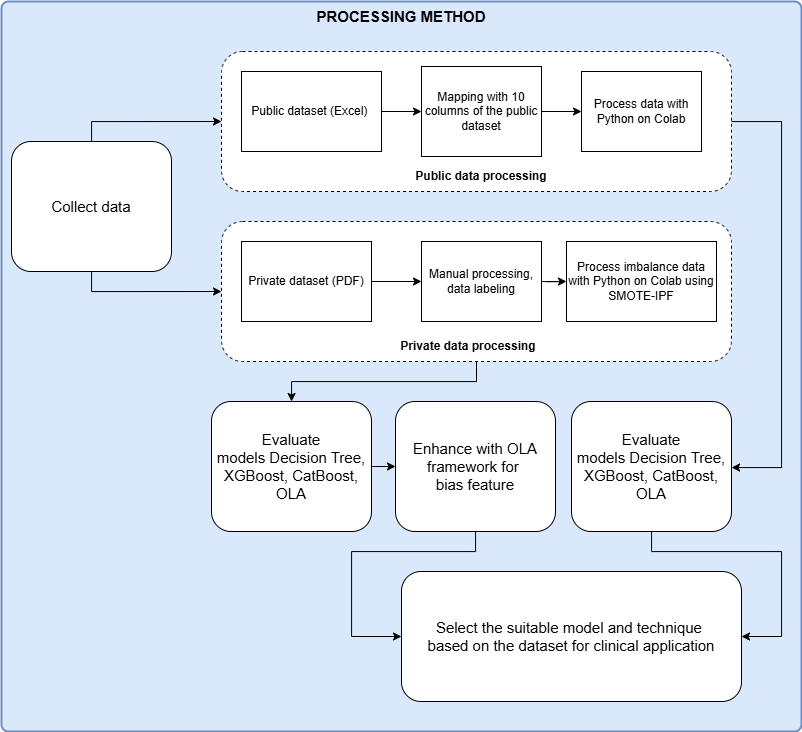
\includegraphics[width=0.95\linewidth]{images/processASD.drawio.png} 
    \caption{Overview of implementation methods}
    \label{fig:ola_pipeline}
\end{figure}

\subsection{Data Preprocessing}
Effective data preprocessing is crucial to ensure the quality and usability of electronic medical records (EMR) for developing an Autism Spectrum Disorder (ASD) screening tool.  
The pipeline comprised five sequential stages, each with a clear \emph{objective} and \emph{method}, as detailed below.

\subsubsection{\textbf{Step 1:} Anonymization}
.

\textit{Objective:} Protect participant privacy. 

\textit{Method:} All personally-identifiable information (e.g., names, ID numbers) was either encrypted or removed before model training.

\subsubsection{\textbf{Step 2:} Redundant Column Removal}
.

\textit{Objective:} Reduce noise and data complexity.

\textit{Method:} Columns lacking analytical value-such as purely administrative metadata-were eliminated.

\subsubsection{\textbf{Step 3:} Missing Value Imputation}
.

\textit{Objective:} Ensure data completeness.

\textit{Method:} Numerical attributes were imputed with the median, while categorical attributes were filled with the mode; domain-expert psychology rules guided these choices where appropriate.

\subsubsection{\textbf{Step 4:} Feature Encoding}
.

\textit{Objective:} Convert categorical data to numerical format suitable for machine learning. 

\textit{Method:}
\begin{itemize}[noitemsep, topsep=2pt]
    \item Target variable (ASD diagnosis) was encoded as binary - \texttt{0} (non-ASD) and \texttt{1} (ASD). 
    \item Behavioral features were encoded as binary (\texttt{0}/\texttt{1}) or ordinal values (\texttt{0}, \texttt{0.5}, \texttt{1}).
\end{itemize}

\subsubsection{\textbf{Step 5:} SMOTE-IPF Balancing}
.

\textit{Objective:} Mitigate class imbalance between ASD and non-ASD cases. 

\textit{Method:} SMOTE was applied to generate synthetic ASD samples via interpolation of feature vectors. Iterative Proportional Fitting (IPF) was then used to eliminate noisy synthetic instances. Unsafe non-ASD samples flagged via KNN-based neighborhood voting were relabeled as ASD to improve balance. This process was repeated iteratively for refinement.

\vspace{0.5em}
Based on domain knowledge, SMOTE-IPF (Synthetic Minority Oversampling Technique with Iterative Partitioning Filter)~\cite{b6} was ultimately selected due to its superior performance in both class balancing and noise reduction.

In contrast, SMOTE-KNN ~\cite{b7} focuses on handling missing values before oversampling. It first imputes missing features using KNN, then applies SMOTE. However, it lacks a mechanism to remove borderline/unsafe samples, potentially introducing noise.

To further enhance training quality, unsafe ASD samples (flagged as negative) were selectively amplified via KNN-based resampling. This produced three datasets:
\begin{itemize}
    \item A0: Baseline dataset after SMOTE-IPF.
    \item A1: Unsafe ASD samples were fully amplified.
    \item A2: Selective amplification based on neighborhood voting.
\end{itemize}

These datasets were exported in Excel format for subsequent model training. Empirical results showed that SMOTE-IPF consistently produced better class balance with reduced overfitting, making it the preferred preprocessing strategy.

\subsection{Classification Models}

\subsubsection{Decision Tree Model}
.

A hierarchical structure of binary decisions based on feature thresholds to classify samples as ASD or non-ASD. Its simplicity and interpretability make it suitable for clinical applications. However, Decision Trees are prone to overfitting, especially on imbalanced datasets, and may overly rely on dominant features, such as specific behavioral indicators, leading to biased predictions. The model was implemented with default parameters, using Gini impurity as the splitting criterion, and evaluated on the preprocessed dataset. Additionally, its performance benefits from pruning techniques to reduce complexity, though it struggles with noisy data and lacks robustness against feature interactions, necessitating careful preprocessing to enhance accuracy in ASD classification.
\subsubsection{XGBoost Model}
.

An ensemble learning method based on gradient boosting, XGBoost integrates multiple weak learners (decision trees) to enhance predictive performance. It effectively manages complex feature interactions and employs regularization to reduce overfitting. However, in imbalanced datasets, XGBoost may favor dominant features, potentially reducing its generalizability in pediatric ASD classification. Additionally, its efficiency stems from parallel processing and optimized tree pruning, though it requires careful hyperparameter tuning to address bias and improve adaptability across diverse data distributions.
\subsubsection{CatBoost Model}
.

CatBoost is an advanced Gradient Boosting Decision Trees (GBDT) algorithm that builds an ensemble of symmetric (oblivious) decision trees to enhance predictive performance and computational efficiency.  
Unlike traditional Decision Trees, CatBoost combines multiple weak learners with ordered boosting and regularization to reduce overfitting, achieving superior generalization on complex datasets. It was configured with a depth of 6 and 100 iterations, leveraging its ability to process ordinal features (e.g., poor-moderate-good encodings) directly.

Compared to Decision Trees, CatBoost excels in handling categorical features through automated label encoding with Bayesian smoothing, eliminating the need for manual preprocessing. Relative to XGBoost, CatBoost offers improved categorical feature processing, optimized GPU performance via histogram-based computations, and automatic feature combinations for complex data patterns.  
However, CatBoost may still struggle with bias toward dominant features in imbalanced datasets, as applied in this study.

\subsubsection{OLA (Overall Local Accuracy)~\cite{b18}}

\paragraph{OLA Model}
OLA is a Dynamic Classifier Selection (DCS) technique from the DESlib library~\cite{b19}, dynamically selecting the most competent classifier for each test sample based on its local accuracy within a region of competence. For each test instance $x$, OLA identifies the $k$-nearest neighbors in the training set, evaluates the classification accuracy of each base classifier on these neighbors, and selects the classifier with the highest local accuracy to predict $x$.

This approach excels in handling complex, heterogeneous, or imbalanced datasets, such as pediatric psychological records, where global models may underperform in specific regions of the feature space. A key strength of OLA is its flexibility in combining diverse base classifiers within a pool.

In this study, OLA was applied to an ensemble comprising DecisionTreeClassifier (simple but prone to overfitting), KNeighborsClassifier (effective in local regions), XGBClassifier (robust boosting for hard samples), and RandomForestClassifier (resilient to overfitting with many features).  
By leveraging local accuracy, OLA dynamically identifies the most suitable classifier for each sample, enhancing fairness and accuracy in ASD classification.

Implemented with custom code to integrate with the SMOTE-IPF preprocessed dataset, OLA mitigates feature bias and improves robustness on imbalanced data. It was hypothesized to outperform the other methods due to its ability to adapt to local data patterns, making it a promising tool for accurate and fair ASD diagnosis in pediatric settings.

\FloatBarrier
\paragraph{Framework with OLA}

This subsection illustrates the enhanced OLA pipeline designed to mitigate feature bias, particularly caused by dominant features such as \texttt{TiepXucMat}: 

\begin{itemize}
\item \textbf{Step 1:} Data Normalization and Dimensionality Reduction with PCA~\\
\textit{Description:} StandardScaler is applied (mean = 0, variance = 1), followed by PCA with $n\_components = 0.95$ to retain 95\% of variance.  
\textit{Output:} Normalized and PCA-transformed data.  
\textit{Purpose:} Reduces noise and dominant feature bias while preserving essential structure.

\item \textbf{Step 2:} Create 3 Diverse Classifier Pools~\\
\textit{Description:}  
\begin{itemize}
    \item Group 1 (PCA-based): DecisionTreeClassifier, XGBClassifier trained on PCA data.  
    \item Group 2 (Bias-controlled): RandomForestClassifier trained on raw data excluding \texttt{TiepXucMat}.  
    \item Group 3 (Raw): KNeighborsClassifier ($k=5$) trained on raw data.
\end{itemize}
\textit{Purpose:} Provides model diversity and flexibility in selection.

\item \textbf{Step 3:} Local Accuracy Estimation and Training OLA Model~\\
\textit{Description:} OLA is trained using Group 1 and selects the most competent classifier for each instance based on KNN-local accuracy.  
\textit{Output:} Trained OLA model using PCA-transformed data.  
\textit{Purpose:} Improves fairness in predictions by choosing locally optimal models.

\item \textbf{Step 4:} Prediction Probabilities from All Model Groups~\\
\textit{Description:}  
\begin{itemize}
    \item OLA produces predictions ($y\_pred$) using Group 1.  
    \item All models output probability estimates via \texttt{predict\_proba}.  
    \item Probabilities are averaged into a final score $y\_prob$.
\end{itemize}
\textit{Purpose:} Mitigates influence of any single biased group; improves ensemble reliability for metrics like ROC AUC.
\end{itemize}


\begin{figure}[H]
    \centering
    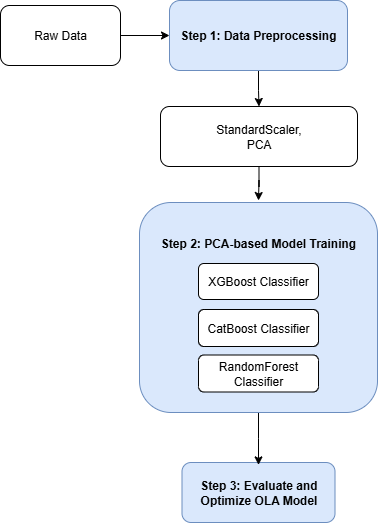
\includegraphics[width=0.95\linewidth]{images/structure_imp_ola.png} 
    \caption{Framework OLA}
    \label{fig:ola_pipeline}
\end{figure}



\subsection{Evaluation Metrics and Validation}

This section defines the evaluation metrics and validation techniques used to assess the performance of the proposed Overall Local Accuracy (OLA) model, alongside Decision Tree, XGBoost, and CatBoost, on the preprocessed ASD dataset.

\subsubsection{Evaluation Metrics} Recall, Specificity, Precision, F1-score

Prioritizing the Recall (sensitivity) metric is driven by the primary goal of maximizing the detection of ASD cases, even if it results in some false negatives. This is particularly critical because missing a diagnosis of ASD in a child can lead to a lack of early intervention, potentially causing severe long-term developmental impacts. Recall measures the proportion of actual ASD cases correctly identified by the model, making it a preferred metric over Precision, F1-score. Even the low Specificity but high Recall is still rated as a suitable model.

\subsubsection{Validation Techniques}


\paragraph{Cross-Validation}

A 5-fold stratified cross-validation was conducted.  

Process: The dataset was divided into 5 folds with preserved class distribution. Each fold was used once as test while others served as training.  

\paragraph{Feature Importance Analysis}

Evaluates the influence of original features on the model's predictions, providing insights into feature relevance for the ASD classification task.

Process: The importance scores of each original feature were computed using the model's built-in feature importance method. These scores were extracted for all features, ranked in descending order based on their contribution, and summed to reflect their overall impact. The results were visualized to highlight the most influential features, aiding in understanding feature bias, such as from the \textit{TiepXucMat} column.


% ---------- CONTINUED SECTIONS ----------


\section{Result and Discussion}
This section presents the key findings from the experiments conducted to evaluate the proposed ASD screening tool, focusing on the performance of the Decision Tree, XGBoost, CatBoost, and enhanced Overall Local Accuracy (OLA) models. The results highlight the effectiveness of the SMOTE-IPF technique and OLA framework in addressing class imbalance and feature bias, with a particular emphasis on achieving high Recall scores to ensure maximum ASD detection.

\subsection{Experimental Results}
This subsection presents the results of the four experimental steps, including performance metrics for all models on both datasets, feature importance analysis, and the impact of the enhanced OLA model. The results are reported using single-run evaluations, 5-fold cross-validation, and visualizations.

\subsubsection{Evaluation Balancing Private Dataset}
.

Two chart 2D PCA visualization bellow reveal that SMOTE-IPF yields a more uniform distribution compared to SMOTE-KNN, with synthetic samples exhibiting tighter clustering and reduced overlap between classes. This indicates SMOTE-IPF’s higher reliability in balancing the private dataset while preserving class separability, enhancing the robustness of subsequent model training.\\
Therefore, private dataset with SMOTE-IPF over 800 records were balanced used for model.

\begin{figure}[H]
    \centering
    \begin{subfigure}[b]{0.48\linewidth}
        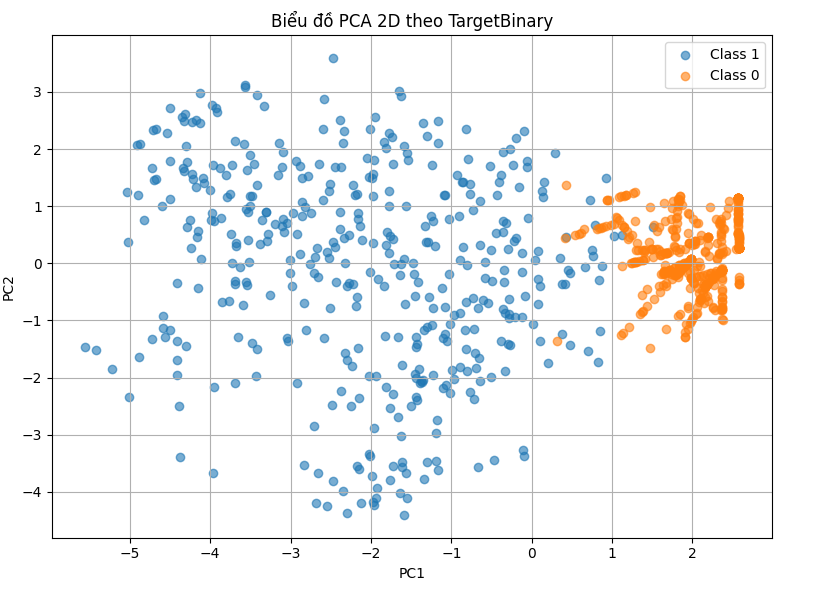
\includegraphics[width=\linewidth]{images/pca_smote_knn.png}
        \caption{PCA with SMOTE-KNN}
        \label{fig:pca-smote-knn}
    \end{subfigure}
    \hfill
    \begin{subfigure}[b]{0.48\linewidth}
        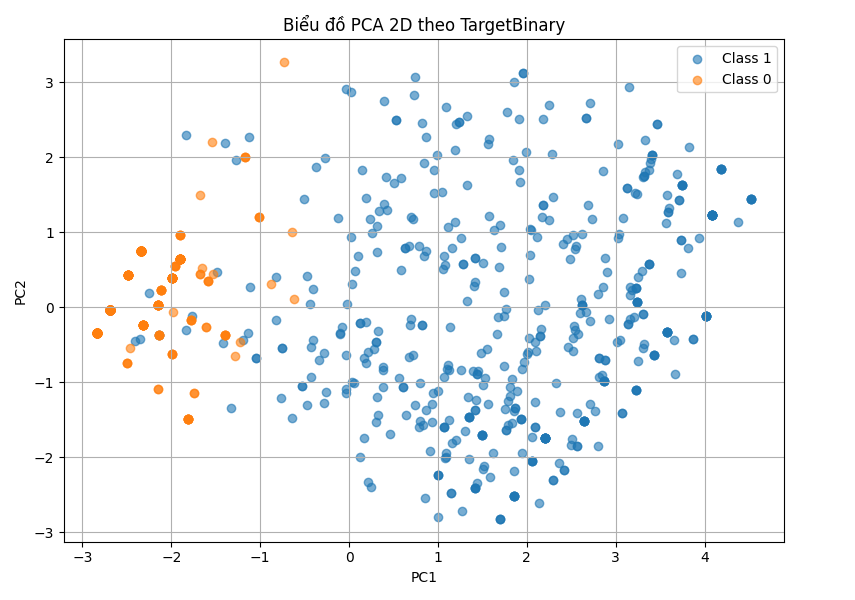
\includegraphics[width=\linewidth]{images/pca_smote_ipf.png}
        \caption{PCA with SMOTE-IPF}
        \label{fig:pca-smote-ipf}
    \end{subfigure}
    \caption{Comparison of PCA visualizations on private dataset using SMOTE-KNN and SMOTE-IPF.}
    \label{fig:pca-comparison}
\end{figure}

\subsubsection{Evaluation on Public and Private Datasets}
\paragraph{Public Dataset}\mbox{}\\
a1) Metrics Cross Validation: \\
% \begin{itemize}
Observations on Performance Metrics\\

- The Decision Tree model yields moderately low results, performing the least effectively among the evaluated models.

- CatBoost delivers good performance, though it is slightly outperformed by XGBoost, with a minimal difference of approximately 0.01.

- XGBoost exhibits very strong results, demonstrating high effectiveness.

- Overall Local Accuracy (OLA) model also achieves very good performance, showcasing its adaptability to the data and surpassing both XGBoost and CatBoost in overall outcomes.

General comment, the Online Learning Algorithm (OLA) demonstrates superior effectiveness, with exceptional adaptability and high accuracy, positioning it as a highly promising model for deployment and further development on real-world datasets. XGBoost and CatBoost are also robust choices, with XGBoost slightly outperforming CatBoost by a marginal difference, indicating their strength in handling complex predictive tasks. Conversely, the Decision Tree model exhibits the lowest performance, making it more suitable for simpler problems or scenarios where model interpretability is prioritized over predictive power.
\begin{table}[H]
\caption{Cross-validation performance (Public dataset)}
\label{tab:cv-public}
\centering
\small
\setlength{\tabcolsep}{4pt}
\renewcommand{\arraystretch}{1.1}
\begin{tabular}{|l|c|c|c|c|c|}
\hline
\textbf{Model} & \textbf{Fold} & \textbf{Recall} & \textbf{Specificity} & \textbf{Precision} & \textbf{F1-Score} \\
\hline
\multirow{6}{*}{Decision Tree}
& 1 & 0.895 & 0.714 & 0.680 & 0.773 \\
& 2 & 0.842 & 0.893 & 0.842 & 0.842 \\
& 3 & 0.789 & 0.714 & 0.842 & 0.714 \\
& 4 & 0.889 & 0.857 & 0.800 & 0.842 \\
& 5 & 0.684 & 0.893 & 0.842 & 0.743 \\
& \textbf{Mean} & \textbf{0.820} & \textbf{0.813} & \textbf{0.757} & \textbf{0.783} \\
\hline

\multirow{6}{*}{XGBoost}
& 1 & 1.000 & 0.929 & 0.957 & 0.950 \\
& 2 & 0.947 & 0.964 & 0.947 & 0.947 \\
& 3 & 1.000 & 1.000 & 1.000 & 1.000 \\
& 4 & 1.000 & 0.857 & 0.818 & 0.900 \\
& 5 & 0.947 & 1.000 & 1.000 & 0.973 \\
& \textbf{Mean} & \textbf{0.979} & \textbf{0.950} & \textbf{0.944} & \textbf{0.954} \\
\hline

\multirow{6}{*}{CatBoost}
& 1 & 1.000 & 0.857 & 0.826 & 0.905 \\
& 2 & 1.000 & 0.964 & 0.950 & 0.974 \\
& 3 & 0.895 & 1.000 & 1.000 & 0.944 \\
& 4 & 1.000 & 0.893 & 0.857 & 0.923 \\
& 5 & 0.947 & 0.963 & 0.947 & 0.947 \\
& \textbf{Mean} & \textbf{0.968} & \textbf{0.935} & \textbf{0.916} & \textbf{0.939} \\
\hline

\multirow{6}{*}{OLA}
& 1 & 1.000 & 1.000 & 1.000 & 1.000 \\
& 2 & 1.000 & 0.964 & 0.959 & 0.979 \\
& 3 & 1.000 & 1.000 & 1.000 & 1.000 \\
& 4 & 1.000 & 0.964 & 0.947 & 0.973 \\
& 5 & 0.947 & 1.000 & 1.000 & 0.973 \\
& \textbf{Mean} & \textbf{0.989} & \textbf{0.986} & \textbf{0.979} & \textbf{0.985} \\
\hline
\end{tabular}
\end{table}

a2) Chart Feature Importance Analysis:\\
General comment, the chart results reveal that the dataset lacks significant column bias, resulting in a relatively uniform distribution across features. The models effectively recognize these features and produce graphs with balanced distributions, ranked from best to worst in a single run as follows: CatBoost - OLA - XGBoost - Decision Tree. OLA and CatBoost demonstrate superior column recognition compared to XGBoost and Decision Tree.

\begin{figure}[H]
    \centering
    \begin{subfigure}[b]{0.45\linewidth}
        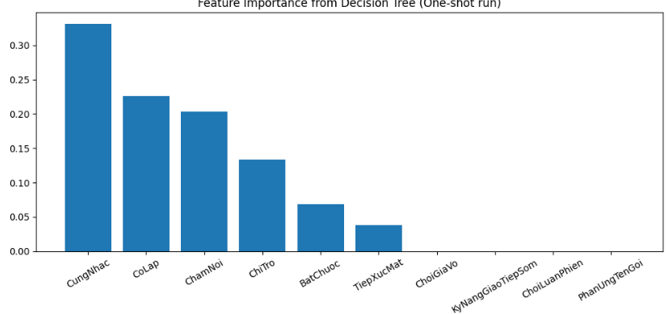
\includegraphics[width=\linewidth]{images/tree_cot.png}
        \caption{Decision Tree}
        \label{fig:x1}
    \end{subfigure}
    \hfill
    \begin{subfigure}[b]{0.45\linewidth}
        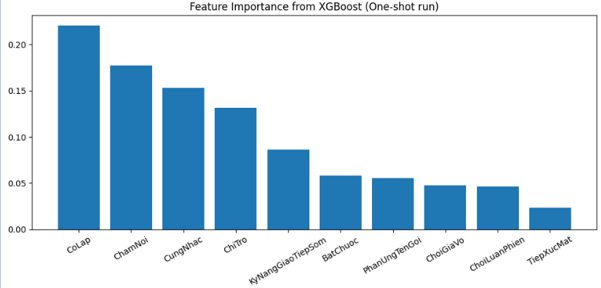
\includegraphics[width=\linewidth]{images/xgb_cot.png}
        \caption{XGBoost}
        \label{fig:x2}
    \end{subfigure}

    \vspace{1em}

    \begin{subfigure}[b]{0.45\linewidth}
        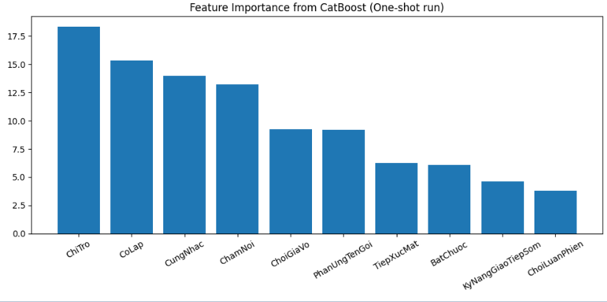
\includegraphics[width=\linewidth]{images/cat_cot.png}
        \caption{CatBoost}
        \label{fig:x3}
    \end{subfigure}
    \hfill
    \begin{subfigure}[b]{0.45\linewidth}
        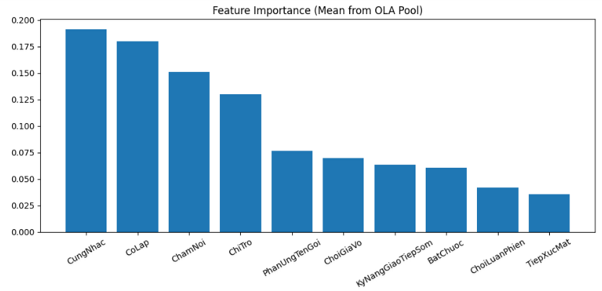
\includegraphics[width=\linewidth]{images/ola_cot.png}
        \caption{OLA}
        \label{fig:x4}
    \end{subfigure}

    \caption{Baseline feature importance in public dataset}
    \label{fig:baseline_features}
\end{figure}


\paragraph{Private Dataset}\mbox{}\\
b1) Metrics Cross Validation: \\

The empirical evaluation of the machine learning models on the real-world dataset highlights their varying performance under conditions of data instability. 

- The Decision Tree model maintains a moderate performance, consistent with its predictions on standardized datasets, but remains the least effective among the evaluated models. 

- CatBoost, while demonstrating good performance, exhibits a notable decline compared to its predictions on standardized datasets. This reduction is attributed to the instability of the dataset and CatBoost's suitability for larger, more stable datasets. 

- XGBoost, initially predicted to yield excellent results, achieves a good performance with a metric of 0.9, outperforming both Decision Tree and CatBoost, though it falls short of its anticipated excellence due to data variability. 

General comment, the Overall Local Accuracy (OLA) delivers outstanding performance, surpassing other models on this real-world dataset. Despite a slight reduction in metrics compared to predictions (approximately 0.02), OLA's adaptability to the unstable data from the clinical setting is evident, outperforming XGBoost and CatBoost in flexibility. Notably, the OLA Framework shows no significant improvement over traditional OLA, with evaluation metrics remaining comparable or exhibiting minimal differences.

These findings suggest that OLA is the most suitable model for datasets lacking stability and clear trends, as encountered in this study. However, potential biases in the dataset's feature columns may contribute to the observed instability, warranting further investigation to mitigate such issues in future applications.
\begin{table}[H]
\caption{Cross-validation performance (Private dataset)}
\label{tab:private_cv_updated}
\centering
\small
\setlength{\tabcolsep}{4pt}
\renewcommand{\arraystretch}{1.1}
\begin{tabular}{|l|c|c|c|c|c|}
\hline
\textbf{Model} & \textbf{Fold} & \textbf{Recall} & \textbf{Specificity} & \textbf{Precision} & \textbf{F1-Score} \\
\hline
\multirow{6}{*}{Decision Tree} 
& 1 & 0.920 & 0.820 & 0.836 & 0.876 \\
& 2 & 0.760 & 0.940 & 0.927 & 0.835 \\
& 3 & 0.840 & 0.840 & 0.840 & 0.840 \\
& 4 & 0.880 & 0.740 & 0.772 & 0.822 \\
& 5 & 0.740 & 0.840 & 0.822 & 0.779 \\
& \textbf{Mean} & \textbf{0.828} & \textbf{0.836} & \textbf{0.839} & \textbf{0.830} \\
\hline

\multirow{6}{*}{XGBoost}
& 1 & 0.920 & 0.900 & 0.902 & 0.911 \\
& 2 & 0.940 & 0.960 & 0.959 & 0.949 \\
& 3 & 0.900 & 0.900 & 0.900 & 0.900 \\
& 4 & 0.960 & 0.840 & 0.857 & 0.906 \\
& 5 & 0.800 & 0.880 & 0.870 & 0.833 \\
& \textbf{Mean} & \textbf{0.904} & \textbf{0.896} & \textbf{0.898} & \textbf{0.900} \\
\hline

\multirow{6}{*}{CatBoost}
& 1 & 0.900 & 0.880 & 0.882 & 0.891 \\
& 2 & 0.920 & 1.000 & 1.000 & 0.958 \\
& 3 & 0.920 & 0.920 & 0.918 & 0.909 \\
& 4 & 0.940 & 0.780 & 0.810 & 0.870 \\
& 5 & 0.820 & 0.880 & 0.872 & 0.845 \\
& \textbf{Mean} & \textbf{0.896} & \textbf{0.892} & \textbf{0.896} & \textbf{0.895} \\
\hline

\multirow{6}{*}{OLA}
& 1 & 0.940 & 1.000 & 1.000 & 0.969 \\
& 2 & 0.980 & 1.000 & 1.000 & 0.990 \\
& 3 & 1.000 & 1.000 & 1.000 & 1.000 \\
& 4 & 0.980 & 0.980 & 0.980 & 0.980 \\
& 5 & 0.920 & 1.000 & 1.000 & 0.958 \\
& \textbf{Mean} & \textbf{0.964} & \textbf{0.996} & \textbf{0.996} & \textbf{0.979} \\
\hline

\multirow{6}{*}{Fw OLA}
& 1 & 0.969 & 0.973 & 0.979 & 0.974 \\
& 2 & 0.980 & 0.973 & 0.980 & 0.980 \\
& 3 & 0.969 & 0.987 & 0.990 & 0.979 \\
& 4 & 0.980 & 0.987 & 0.990 & 0.985 \\
& 5 & 0.938 & 1.000 & 1.000 & 0.968 \\
& \textbf{Mean} & \textbf{0.967} & \textbf{0.984} & \textbf{0.988} & \textbf{0.977} \\
\hline
\end{tabular}
\end{table}

b2) Chart Feature Importance Analysis:\\
The bias column evaluation charts reveal the following insights:

The dataset exhibits a significant bias toward the "TiepXucMat" (Eye Contact) column across all four models, leading to overly optimistic evaluation metrics. However, when applied to new datasets in real-world scenarios, the results fall short of expectations if the "TiepXucMat" column is not accurately assessed.

Although CatBoost shows lower Cross Validation performance compared to other models, it maintains a better distribution of the biased column. However, it cannot be conclusively regarded as the best model for column distribution.

OLA remains a promising model for further improvement due to its flexible adaptability.

General comment, the dataset is predominantly biased toward the "TiepXucMat" column, necessitating enhancements to the adaptable OLA model. These improvements should aim to achieve a more uniform and balanced differentiation across columns, ensuring that the screening process does not miss positive cases.
\begin{figure}[H]
    \centering
    \begin{subfigure}[b]{0.45\linewidth}
        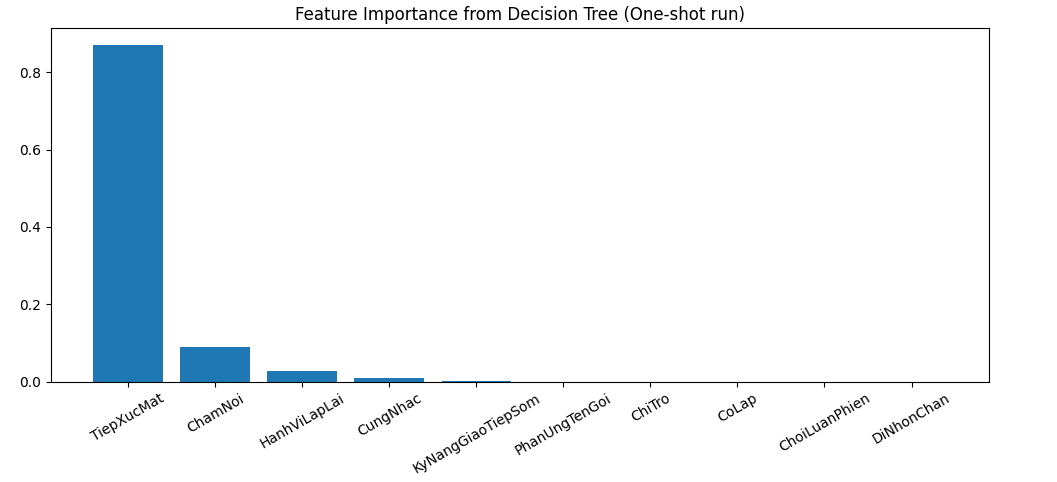
\includegraphics[width=\linewidth]{images/feature_dt.png}
        \caption{Decision Tree}
        \label{fig:x1}
    \end{subfigure}
    \hfill
    \begin{subfigure}[b]{0.45\linewidth}
        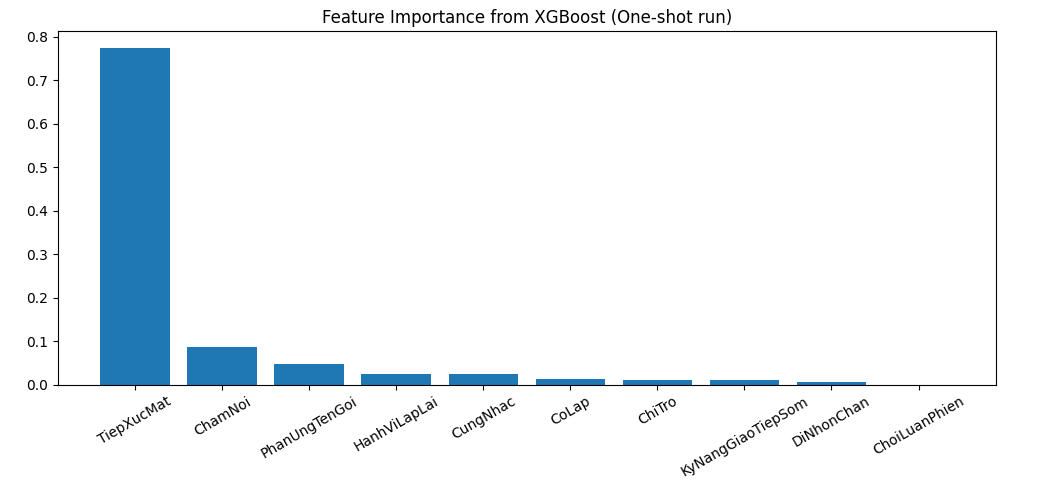
\includegraphics[width=\linewidth]{images/feature_xgb.png}
        \caption{XGBoost}
        \label{fig:x2}
    \end{subfigure}

    \vspace{1em}

    \begin{subfigure}[b]{0.45\linewidth}
        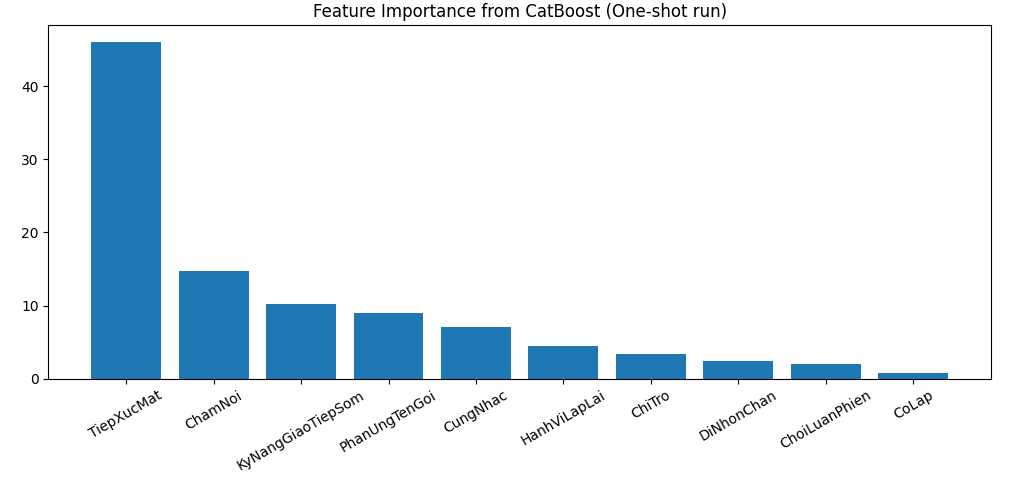
\includegraphics[width=\linewidth]{images/feature_cat.png}
        \caption{CatBoost}
        \label{fig:x3}
    \end{subfigure}
    \hfill
    \begin{subfigure}[b]{0.45\linewidth}
        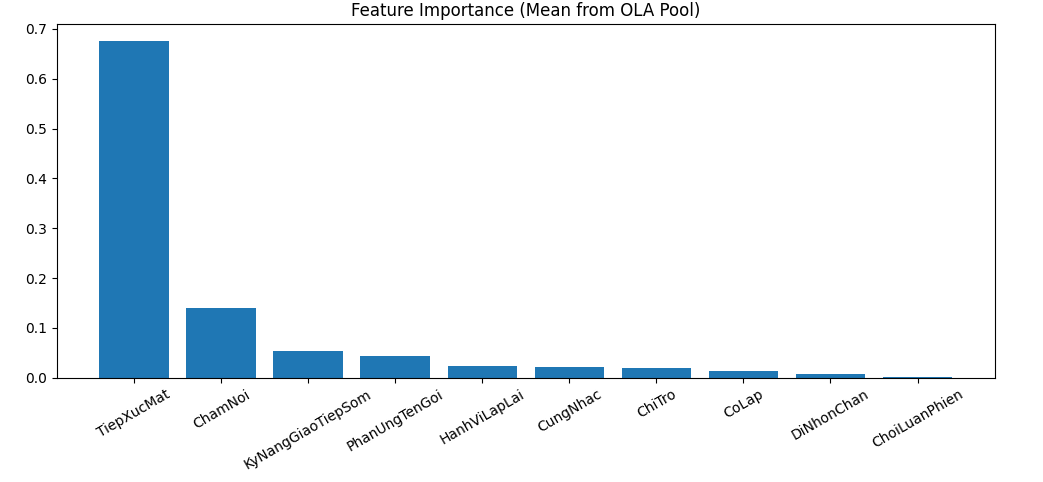
\includegraphics[width=\linewidth]{images/feature_ola.png}
        \caption{Initial OLA}
        \label{fig:x4}
    \end{subfigure}

    \caption{Baseline feature importance in private dataset}
    \label{fig:baseline_features}
\end{figure}

To address this, Enhanced OLA was applied to reduce bias and diversify feature influence.

\begin{figure}[H]
    \centering
    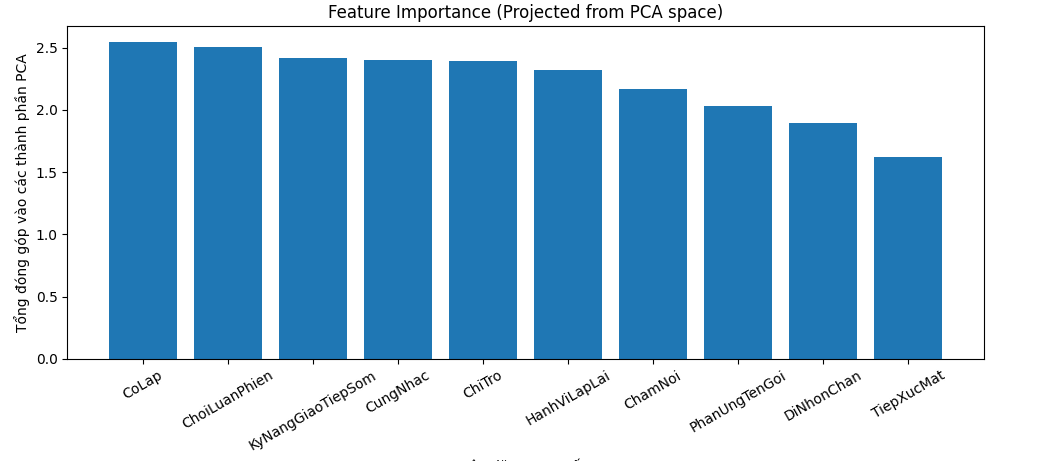
\includegraphics[width=0.85\linewidth]{images/feature_enhanced_ola.png}
    \caption{Enhanced OLA framework with TiepXucMat}
    \label{fig:importance_after}
\end{figure}

\noindent\textbf{Summary:} Enhanced OLA framework successfully reduced the dominance of \textit{TiepXucMat}, improving balance among features and robustness for ASD classification on the private dataset.
% \end{itemize}

\subsection{Discussion}
This section analyzes the performance patterns across the evaluated models, discusses the improvements of OLA's local selection mechanism over global bias, compares our results with related work, and highlights limitations, strengths, weaknesses, and the practical applicability of OLA on the private dataset.

\begin{table}[ht]
\caption{Compare Recall on public and private datasets}
\label{tab:recall_public_private}
\centering
\small                 % thu nhỏ font để vừa cột
\setlength{\tabcolsep}{6pt} % thu hẹp khoảng cách cột
\renewcommand{\arraystretch}{1.1} % dãn dòng nhẹ
\begin{tabular}{|l|c|c|}
\hline
\textbf{Model} & \textbf{Public} & \textbf{Private} \\
\hline
Decision Tree & 0.820 & 0.828 \\
XGBoost       & 0.979 & 0.904 \\
CatBoost      & 0.968 & 0.896 \\
OLA           & 0.989 & 0.964 \\
OLA Framework & --\footnotemark & 0.967 \\
\hline
\end{tabular}
\end{table}

\footnotetext{OLA Framework doesn't need to be assessed on public dataset so “--”.}

Compare Recall on public and private datasets, as depicted in the provided table, highlight the performance of various machine learning models across public and private datasets, with a focus on Recall as the primary metric due to its importance in ensuring maximum detection of ASD cases. The table shows that OLA and the OLA Framework in practical data achieved the highest Recall scores of 0.964 and 0.967, respectively, significantly outperforming CatBoost (0.896), XGBoost (0.904), and Decision Tree (0.828). This superior performance underscores OLA's exceptional flexibility in dynamically selecting optimal models, reinforcing its robustness and adaptability across diverse datasets.

A notable observation is the decline in accuracy when these models are applied to the private clinical dataset compared to the public dataset. XGBoost dropped from 0.979 to 0.904, CatBoost from 0.968 to 0.896, and OLA from 0.989 to 0.964-a reduction of only 0.025. This decrease indicates that while all models perform well (above 0.9 on average), their effectiveness diminishes in real-world settings with unstable data, failing to replicate the high accuracy observed in controlled experiments. The private dataset's variability reflects the challenges of real-world clinical environments, where data inconsistencies are common.

Further analysis of column bias reveals a significant skew toward the "TiepXucMat" (Eye Contact) column in the private dataset, which likely contributed to the overly optimistic results in initial evaluations. This bias suggests that the models' predictions may overly rely on a single feature, potentially leading to inaccurate assessments when applied practically. The OLA Framework was introduced to address this limitation, balancing feature weights and integrating the 10-question framework across 10 screening themes. Post-implementation, the OLA Framework successfully mitigated this bias, still achieving a Recall of 0.967, demonstrating its ability to adapt to real-world data fluctuations.

\section{Conclusion}
\subsection{Results achieved}

\begin{figure}[H]
    \centering
    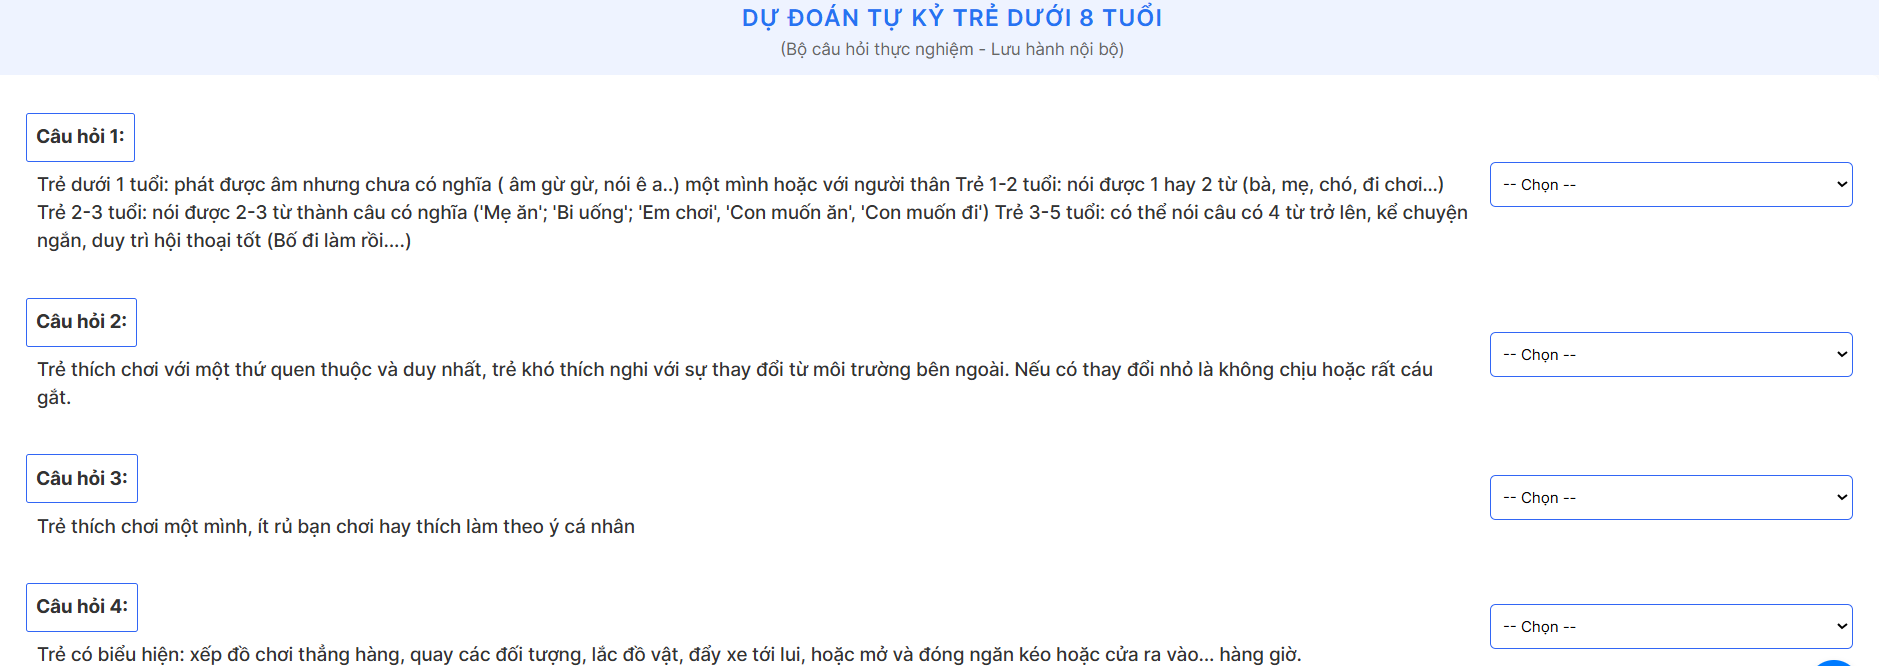
\includegraphics[width=0.85\linewidth]{images/screen.png}
    \caption{Overview of autistic screening software}
    \label{fig:importance_after}
\end{figure}
\subsection{Conclusion}

This study introduces a screening tool leveraging machine learning models trained on psychological medical records of children, utilizing the Overall Local Accuracy (OLA) framework following advanced preprocessing techniques. These include balancing class labels with SMOTE-IPF and mitigating column bias through the OLA framework. Traditional models, including advanced ones like CatBoost, struggled with imbalanced data, facing limitations due to a "column causing data bias" that undermined reliability, particularly given the hidden biases often present in real-world datasets. The enhanced OLA, equipped with additional techniques to control this bias, proved to be a robust solution, significantly improving ASD case detection and ensuring stable performance.
The primary contribution of this research is a novel approach to developing an ASD screening tool, with potential applicability to screening other medical conditions using psychological medical records and machine learning. This work lays the groundwork for more accurate, equitable, and user-friendly diagnostic tools, particularly for early screening where missing cases are a critical concern. However, challenges remain, including the limited dataset size and the unreliable nature of manual labeling. Future efforts should focus on testing the OLA framework on larger datasets, validated through real-world software trials combined with corresponding medical records to further train the model. This approach will ensure the capture of outlier cases and enable broader scalability, extending the tool’s use beyond a single clinic to multiple healthcare facilities and hospitals nationwide. The OLA Framework’s strength lies in its dynamic model selection and adaptability, making it highly suitable for building ASD screening tools in the context of volatile real-world datasets. Its ability to maintain high performance despite data instability and column bias positions it as an ideal solution for clinical applications, especially in resource-constrained settings where robust and flexible tools are vital. Future enhancements should prioritize refining feature weighting to improve generalizability across diverse populations.

\section{Acknowledgment}
We would like to express our sincere gratitude to the University of Information Technology, Vietnam National University Ho Chi Minh City (UIT, VNU-HCM), for their support and for providing the necessary resources throughout this research. This research was supported by The VNUHCM-University of Information Technology’s Scientific Research Support Fund.\\

We also would like to thank experts in the field of psychological health for providing young medical record data and professional documents, who supported the research team to authenticate and consolidate professional knowledge so that the group can achieve the best research results.

% ---------- REFERENCES ----------
\begin{thebibliography}{99}
\bibitem{b1} Holly Hodges, Casey Fealko, Neelkamal Soares. "Autism spectrum disorder: definition, epidemiology, causes, and clinical evaluation", 2020. doi: https://doi.org/10.21037/tp.2019.09.09

\bibitem{b2} Bang Le. "Ty le tre tu ky o Viet Nam va The gioi: Nhung con so bao dong", 2025. url: https://tretuky.edu.vn/ty-le-tre-tu-ky-o-viet-nam-va-the-gioi/

\bibitem{b3} Clara Lucato dos Santos, Indyanara Inacio Barreto, Idevaldo Floriano, Luca Schiliró Tristao, Antonio Silvinato, Wanderley Marques Bernardo. "Screening and diagnostic tools for autism spectrum disorder: Systematic review and meta-analysis", March 2024. doi: https://doi.org/10.1016/j.clinsp.2023.100323

\bibitem{b4} Paul Olubudo. "Statistical Bias Correction in Imbalanced Datasets", April 2025. doi: https://www.researchgate.net/publication/390805682

\bibitem{b5} Harshita Chandrappa, Swaathi BR, Prof. Swimpy Pahuja. ``Prediction of Autism Spectrum Disorder based on Machine Learning Approach,'' \textit{International Journal for Research in Applied Science \& Engineering Technology (IJRASET)}, vol. 11, no. V, pp. 3521-3526, May 2023. doi: 10.22214/ijraset.2023.52417. Available: \url{https://doi.org/10.22214/ijraset.2023.52417}

\bibitem{b6} J. A. Sáez, J. Luengo, J. Stefanowski, and F. Herrera, ``A novel technique for text classification using SMOTE-IPF based oversampling and deep neural network'' \textit{Int. J. of Advanced Computer Science and Applications}, vol. 12, no. 10, 2014. doi: 10.14569/IJACSA.2021.051.

\bibitem{b7} H. Karamti \textit{et al.}, ``SMOTE-KNN: An improved algorithm based on SMOTE and K-nearest neighbors for imbalanced data,'' \textit{IEEE Access}, vol. 9, pp. 95690--95701, 2023. doi: 10.1109/ACCESS.2023.5174412.

\bibitem{b8} B. D. Hung, V. V. Thoa, and X. T. Dang, ``KSI - A combined clustering and resampling method with noise filtering algorithm for imbalanced data classification,'' \textit{J. of Information and Communication Technology}, vol. 1, no. 1, pp. xx--xx, 2019.

\bibitem{b9} Y. Hong and E. Yang, ``Unbiased classification through bias-contrastive and bias-balanced learning,'' in \textit{Advances in Neural Information Processing Systems (NeurIPS)}, vol. 34, pp. 20153--20165, 2021.

\bibitem{b10} Z. Liu \textit{et al.}, ``Ola: Pushing the frontiers of omni-modal language model with progressive modality alignment,'' \textit{arXiv preprint}, arXiv:2502.04328, 2025. Available: \url{https://arxiv.org/abs/2502.04328}

\bibitem{b11} J. M. Moriuchi, A. Klin, and W. Jones, ``Mechanisms of diminished attention to eyes in autism,'' \textit{Am. J. of Psychiatry}, vol. 173, no. 8, pp. 825--833, 2016. doi: 10.1176/appi.ajp.2016.15081034.

\bibitem{b12} S. Ramos-Cabo, V. Vulchanov, and M. Vulchanova, ``Different ways of making a point: A study of gestural communication in typical and atypical early development,'' \textit{Autism Research}, vol. 14, no. 5, pp. 984--996, 2021. doi: 10.1002/aur.2474.

\bibitem{b13} M. Miller \textit{et al.}, ``Response to name in infants developing autism spectrum disorder: A prospective study,'' \textit{The J. of Pediatrics}, vol. 165, no. 2, pp. 332--337, 2014. doi: 10.1016/j.jpeds.2014.04.017.

\bibitem{b14} M. Montagut-Asunción \textit{et al.}, ``Joint attention and its relationship with autism risk markers at 18 months of age,'' \textit{Children}, vol. 9, no. 4, 2022. doi: 10.3390/children9040480.

\bibitem{b15} B. Ingersoll, ``The social role of imitation in autism: Implications for the treatment of imitation deficits,'' \textit{Infants \& Young Children}, vol. 21, no. 2, pp. 107--119, 2008. doi: 10.1097/01.IYC.0000314482.24087.14.

\bibitem{b16} Y. G. Lam and S. S. Yeung, ``Symbolic play in children with autism,'' in \textit{Comprehensive Guide to Autism}, Springer, 2014, pp. 491--508. doi: 10.1007/978-1-4614-4788-7\_26.

\bibitem{b17} F. F. Tabtah, ``Autism spectrum disorder screening,'' dataset about list 10 question to predict ASD in kaggle in \textit{Proc. 1st Int. Conf. on Medical and Health Informatics}, Taichung City, Taiwan, ACM, 2017. Available: \url{http://fadifayez.com/wp-content/uploads/2017/11/Autism-Spectrum-Disorder-Screening-Machine-Learning.pdf}

\bibitem{b18} Overall Local Accuracy. Available: \url{https://deslib.readthedocs.io/en/latest/modules/dcs/ola.html}

\bibitem{b19} R. M. O. Cruz, R. Sabourin, and G. D. C. Cavalcanti, ``DESlib: A dynamic ensemble selection library in Python,'' 2018. Available: \url{https://github.com/scikit-learn-contrib/DESlib}

\end{thebibliography}


\end{document}
